\chapter{Single-cell mRNA processing}
% This is only a test.
% \section{A section}
% Lorem ipsum dolor sit amet, consectetuer adipiscing elit. Nulla odio
% sem, bibendum ut, aliquam ac, facilisis id, tellus. Nam posuere pede
% sit amet ipsum. Etiam dolor. In sodales eros quis pede.  Quisque sed
% nulla et ligula vulputate lacinia. In venenatis, ligula id semper
% feugiat, ligula odio adipiscing libero, eget mollis nunc erat id orci.
% Nullam ante dolor, rutrum eget, vestibulum euismod, pulvinar at, nibh.
% In sapien. Quisque ut arcu. Suspendisse potenti. Cras consequat cursus
% nulla.

% \subsection{A Figure Example}
% \label{ssec:figure_example}

% This subsection shows a sample figure.

% \begin{figure}[h]
%   \centering
%   \includegraphics[width=0.5\textwidth]{sandiego}
%   \caption[Short figure caption (must be \protect{$< 4$} lines in the list of figures)]{
%   A picture of San Diego.  Note that figures must be on their own line (no neighboring text) and captions must be single-spaced and appear \protect\textit{below} the figure.  Captions can be as long as you want, but if they are longer than 4 lines in the list of figures, you must provide a short figure caption.\index{SanDiego}}
%   \label{fig:sandiego}
% \end{figure}

% \subsection{A Table Example}

% While in Section \ref{ssec:figure_example} Figure \ref{fig:sandiego} we had a majestic figure, here we provide a crazy table example.


% %%%% TABLE 1 %%%%
% \vspace{0.25in}
% \begin{table}[!ht]
% \caption[Short figure caption (must be \protect{$< 4$} lines in the list of tables)]{A table of when I get hungry.  Note that tables must be on their own line (no neighboring text) and captions must be single-spaced and appear \protect\textit{above} the table.  Captions can be as long as you want, but if they are longer than 4 lines in the list of figures, you must provide a short figure caption.}

% \vspace{-0.25in}
% \begin{center}
% \begin{tabular}{|p{1in}|p{2in}|p{3in}|}

% \hline
% Time of day & Hunger Level & Preferred Food \\

% \hline
% 8am & high & IHOP (French Toast) \\

% \hline
% noon & medium & Croutons (Tomato Basil Soup \& Granny Smith Chicken Salad) \\

% \hline
% 5pm & high & Bombay Coast (Saag Paneer) or Hi Thai (Pad See Ew) \\

% \hline
% 8pm & medium & Yogurt World (froyo!) \\

% \hline
% \end{tabular}
% \end{center}
% \label{tab:analysis3}
% \end{table}

\section{Introduction}
The human body contains an estimated $3.72\times 10^{13}$ cells \cite{Bianconi2013-jr}, all of which are highly specialized in form and function, and yet despite their incredible diversity in phenotypes, each cell contains nearly identical genotypes. These cells are heterogeneous because of their different RNA, protein, and metabolite molecules, which coordinately regulate the cell to express precise phenotypes. To study the variation between cells, we turn to single-cell analysis.

The original tool for single-cell analysis is the microscope \cite{Hooke1665-bk,Van_Leeuwenhoek_undated-gu}, which can visualize structural differences between individual cells, but the molecules that create these differences are too small to resolve in live cells by current microscope technology. To compare the molecules of single cells, recent advances in microfluidics have allowed for capture of one cell at a time, which can be coupled with modern high-throughput technology to measure many messenger RNA (mRNA) molecules per cell, and together these are combined to create single-cell RNA-sequencing (scRNA-Seq) \cite{Kolodziejczyk:2015dj,Ziegenhain:2017kr}. Computational analysis of these high-dimensional data can identify distinct cellular states or delineate cellular trajectories [reviewed by \cite{Bacher:2016jq,Cannoodt2016-mt,Liu:2016fd,Trapnell:2015er,Stegle:2015cx}.].

While single-cell capture has enabled probing of cellular state measured through mRNA abundances, the study of an mRNA molecule's rich life (Figure~\ref{fig:singlecell_questions}a) from birth (transcription) to death (degradation), the collection of actions known as mRNA processing \cite{Blanc2003-wk,Gerstberger:2014bx,Yeo:2016vz,Nussbacher:2015cwa,Singh:2015jg}, has only started to be addressed at the single-cell level. As in bulk RNA-seq \cite{Anders:2012esa,Kleinman:2012cu,Lianoglou:2013gw,Nishikura2010-dk,Park:2012hz,Peng2012-ru,Shen:2014gs,Wang:2008gt}, scRNA-seq has enabled the investigation of RNA processing features that are measureable by sequencing, such as alternative splicing, RNA editing, and alternative polyadenylation \cite{Karlsson2017-wy,Marinov2014-iw,Picardi2017-bv,Shalek2013-ez,Velten:2015ie,Welch:2016iz}. However, the high-throughput nature of scRNA-seq captures only the abundance of RNA transcripts in a snapshot in time and loses the information of RNA modifications, dynamics, localization, binding partners, and secondary structure. Thus, these features must be measured a different way.

Ideally, we would capture the entire cellular and molecular context of an RNA molecule. To accomplish this, we turn back to the microscope, a tried and true tool. While even the highest resolution microscopes cannot discern individual molecules without significant amplification \cite{Femino1998-ws,Raj2009-ni}, microscopy captures cellular context including morphology and subcellular localization, and in the case of live-cell imaging, dynamics. Microscopy is limited by the ability to design fluorescent constructs to visualize RNA and protein molecules, and as a result, can only be performed for a few targets a time. Middle-ground technologies that are relatively high-throughput but also measure several aspects of the same cell or same transcript \cite{Gierahn2017-ko,Macaulay2017-tb} have highest potential for discovery.
We will review the available methods to probe RNA processing at the single cell level, and highlight the current limitations, showing opportunities for novel technology to make breakthroughs in the knowledge of RNA processing.

% --- BEGIN manual facingcaption --- %
\clearpage
\thispagestyle{facingcaption}
\begin{figure}[h]
\captionsetup{labelformat=prev-page}
\caption[Overview of open questions in single-cell RNA processing.]{\textbf{Overview of open questions in single-cell RNA processing.}\\
\textbf{a.}~Overview of the processing steps in an RNA's life cycle: transcription (biogenesis), alternative splicing, poly-adenylation, modification, export, localization, translation, and degradation.\\
\textbf{b.}~Dichotomy of investigating distribution of transcripts across cells with high-throughput methods, and distribution of transcripts within cells using high-resolution methods.\\
\textbf{c.}~Examples of high-throughput measurements, where many transcripts can be measured at once, but only one feature of them may be measured.\\
\textbf{d.}~Examples of high-resolution measurements, where only a few transcripts can be measured at once, but many features of them can be profiled.
}
\label{fig:singlecell_questions}
\end{figure}
\clearpage
\begin{figure}[h]
\ContinuedFloat
\captionsetup{labelformat=empty}
\centering
% \includegraphics[width=5.8in]{sandiego.jpg}
\includegraphics[width=5.8in]{figures/singlecell_questions.pdf}
\end{figure}
%and, I'm not sure why, but one of the times I used this code the figure number wasn't augmented for the next figure, so check your figure numbers and if necessary uncomment the following line
%\addtocounter{figure}{1}
\clearpage
% --- END manual facingcaption --- %

% ---- BEGIN "facingcaption" page style - didn't work for me --- %
% % use "facingcaption" page style to put the caption on the left
% \newpage
% \thispagestyle{facingcaption}
% \begin{center}
% \vspace*{3in}
% \textbf{Overview of open questions in single-cell RNA processing.}
% \end{center}
% \textbf{a.}~Overview of the processing steps in an RNA's life cycle: transcription (biogenesis), alternative splicing, poly-adenylation, modification, export, localization, translation, and degradation.\\
% \textbf{b.}~Dichotomy of investigating distribution of transcripts across cells with high-throughput methods, and distribution of transcripts within cells using high-resolution methods.\\
% \textbf{c.}~Examples of high-throughput measurements, where many transcripts can be measured at once, but only one feature of them may be measured.\\
% \textbf{d.}~Examples of high-resolution measurements, where only a few transcripts can be measured at once, but many features of them can be profiled.


% % \end{center}
% \newpage

% \begin{figure}[h]
%   \centering
%   \includegraphics[width=5.8in]{figures/singlecell_questions}
%   \caption[Overview of open questions in single-cell RNA processing.]{Overview of open questions in single-cell RNA processing.}
% \label{fig:singlecell_questions}
% \end{figure}
% ---- END "facingcaption page style - didn't work for me --- %

\section{Balancing high-throughput and high-resolution single-cell technologies}

A complex tissue such as the human brain contains many different transcripts, but by measuring them at the bulk level, the cell of origin for each transcript is unknown (Figure~\ref{fig:singlecell_questions}b, left). Using single-cell technologies, we quantify an RNA processing event either as presence or absence (e.g. m6A or splicing) or a continuous quantity (e.g. abundance or poly-A tail length). With these quantifications in hand, we want to be able to capture individual cells and measure each cell's transcripts to understand two separate questions (Figure~\ref{fig:singlecell_questions}b): How are transcripts distributed (1) across cells, and (2) within cells?
	The questions of distributions of transcripts across cells and within cells represent the ends of a spectrum, each with their own advantages and limitations. Where on the one extreme there are high-throughput methods which can measure many transcripts per cell, but are low-resolution and can only measure one aspect, abundance, and on the other extreme are high-resolution methods which can measure a limited number of transcripts (low-throughput) but can measure many aspects beyond abundance, such as dynamics and localization.


\subsection{Throughput vs resolution}
On the one end, we have high-throughput, low-resolution methods
We define ``throughput'' as the number of different transcript molecules that can be measured at once from a single cell (Figure~\ref{fig:singlecell_questions}c)
Throughput indicates the number of different transcripts that can be measured at once
When we quantify an RNA processing event either as presence or absence (e.g. m6A or splicing) or a continuous quantity (e.g. abundance or poly-A tail length), we want to know about them at the single cell-level: (1) Distribution across cells, within a population, and whether this feature is bimodal or multimodal and can distinguish population substructures. Do these processes co-occur on the same transcript, or on different transcripts within the same cell?
E.g. High-throughput means many things can be measured at once, like RNA-Seq
The enormous amounts of data may sometimes feel like staring into ``tea leaves'' to understand
Requires many computational manipulations, which can pull away from the biology
Farthest away from the biology
High-throughput methods allow for low-resolution studies of many targets
E.g. Only one measurement, but many features
One thing I'm trying to say here echoes Jaron Lanier's ``You are Not a Gadget'' which talks about how as soon as you try to represent something digitally, you are taking away features and things that you never thought to keep
For example, if you wanted to digitize a painting, you may not think to capture the kinds of oils that were used for the paints, where the paints came from, who wove the muslin cloth and who mounted it, the tautness of the cloth mounted to the frame, etc. All kinds of incidental measurements that are lost as soon as you measure it.
I want to make the analogy to high throughput measurements.
As soon as you measure the RNA content of a cell through RNA-seq, you lose all the incidental information, such as its structure and nucleotide modifications, its localization and binding partners, its lifespan, and so on
What's missing:
Dynamics
Snapshot in time
Localization

Interactions
Structure/Modifications
Low-throughput means only one transcript can be measured at once, e.g. RNA-FISH where only a few probes at a time can be visualized
Resolution indicates the number of aspects of an individual transcript that can be measured in a single cell (Figure~\ref{fig:singlecell_questions}d)
To further investigate the subcellular characteristics such as time scales and localization, we want to know (2) the distribution across transcripts, within individual cells. If an RNA processing event occurs only in certain subpopulations, then how does it work in those subpopulations? If it co-occurs in the same cell, how does the cell use the different transcripts differently?
E.g. High-resolution means multiple aspects of a single transcript can be measured
E.g. microscopy-based methods can show dynamics, localization, co-localization with another molecule, biogenesis/degradation, interactions
Can end up observing/measuring things you didn't plan on observing in the first place
Closest to the biology

E.g. low-resolution means only a few aspects of a molecule
E.g. for RNA seq can estimate abundance, splicing, RNA editing
But can't get localization, dynamics, interactions
Low-throughput methods allow for high resolution studies of a few target
One feature, many measurements
Microscopy-based methods are ``single-cell'' and through live cell imaging, allow for observation of many dynamics, localization
While an old tool, the microscope has undergone many advances
This allows for analysis and discovery of characteristics that may be serendipitous or not have been planned, e.g. co-localization with cellular structures or visualization of unique dynamics in certain localizations, e.g. different dynamics in the nucelus vs cytoplasm \cite{Yap:2016bs,Yap:2016ig} is a really great example of this. Both isoforms found in individual neurons
Technologies that balance both throughput and resolution that are ``just right,'' as in the children's fairy tale of ``Goldilocks''
lie in the ``Goldilocks'' middle ground, are a major need and are currently limited in the still-growing field of technological development in single cells
Most technological innovation has focused on increasing throughput or resolution, but we argue that the large leaps will be made by combining the two to show sevearl aspects of a single RNA transcript molecule, in a way that has never been seen before.
in situ sequencing Long Cai's lab \cite{Shah:2016iy}
Combination technologies, from the same cell
The DNA-based ones are good for understanding how DNA mosaicism contributes to gene expression
RNA-seq + DNA-seq
To answer the question of how epigenetics contributes to gene expression, you can use RNA-Seq + methyl-seq
How do RNA levels influence protein levels?
Seq-well (w/antibodies) \cite{Gierahn2017-ko}
STill need:
How do global RNA levels influence global protein levels?
RNA-Seq + Proteomics
How is the same RNA folded into 3D structures within the same cell? How does this change with time and localization?
First, low throughput microscopy-based methods
Eventually: RNA-Seq + RNA Structure
Most high-throughput single cell analyses have been used to study cellular biology, for example, defining cell state as gene expression to delineate cellular trajectories \cite{Cannoodt2016-mt}.
however the resolution of the microscope is such that we can see subcellular organelles, but not molecules.
WHile the microscope is great for cellular biology, cannot use it to study molecular biology
However, single cell analyses can be used to study molecular processes,
Initial studies were about how genes or RNA processing events are distributed across a population
Later, will interrogate how RNA processing is distributed within a cell
Ultimately, ‘single-cell biology' is ‘biology'
However, modern tools for ``single-cell analysis'' couple a high-throughput single-cell capture method, usually based in microfluidics, and a high-throughput measurement tool such as RNA-seq \cite{Ziegenhain:2017kr} or antibody-based mass cytometry \cite{Bendall2011-jm}
However, there are much older tools for performing single cell analysis - the microscope, FACS

RNA molecules lead rich and fulfilling lives, and yet we have little idea what the entire life cycle for a single RNA looks like or how to track it.
RNA processing has extensively been reviewed [citations]
What we want to know about RNA processing events at the single cell level:


Quantification: Presence or absence (e.g. m6A), or continuous quantity (e.g. length of poly-A tail)
(1) Distribution across cells, within a population - cellular biology
Population substructure
Bi- and multi-modality
Does these processes co-occur in the same cell, or are they in different cells?
How can you be sure?
How does this RNA processing event affect cellular fate?
Since only get a snapshot, need to follow up with an experiment that turns the process off, or that overexpresses the process, to see how it affects cell fate
Hypothesis-generating
Before:
Bulk sequencing lets us see some trends and make correlations
E.g. methylation of a particular site is correlated with expression (??? - I made this up)
Now:
Single-cell sequedncing lets you see the entire spectrum of variation, for one measurement
Distribution across transcripts, within cells - molecular biology
Does these processes co-occur on the same transcript, or on different transcripts within the same cell?
Maybe could be answered by high-throughput manner
How does this RNA processing event work?
Localization
Structure
Interactions
RNA pull down
``Single-cell biology -- isn't that what we've been calling ‘biology' for decades?'' \cite{Symmons2016-xn}

Common themes
Heterogeneity
Tissues
How systems work
But measuring individual systems
Mosaicism
E.g. X-inactivation → is it always the same X-chromosome that gets inactivated? (no, female calico cats)
Is this really different from heterogeneity?
What is ``noise'' and what is functional? Maybe the noise itself is functional?

Currently, the phrase ``single-cell analysis'' tends to mean in modern times, high-throughput single cell capture and measurement such as RNA-Seq.


\subsection{In vitro vs in vivo}
In vitro
good for developing computational models
Since they're seemingly homogeneous populations
Good for understanding molecular biology
Somewhat of a ``gold standard''
Controlled population
Can Look at partitioning of transcriptome between daughter cells
Intermediate: organoids
Good for studying cellular and organ-level biology in a controlled system
Still don't know exact mapping to the true organ system
In vivo
good for understanding organism-level cellular biology, fully within the context of the samples
If there existed a perfect cell-type classifier, then in vivo could also be used to classify cells, then study their differential RNA processing
To measure RNA processing across cells, we use high-throughput single-cell technologies to study cellular biology and answer the question, is a particular RNA processing event found only within certain subpopulations of cells, or does it co-occur within individual cells? If it's found within the same cell, are these on the same transcript, or on different transcripts in individual cells? Since these technologies only extract a snapshot in cellular time, akin to a still frame in a movie, we don't know how these transcripts change over time or how they are physically used within an individual cell, and thus high-throughput technologies are hypothesis-generating experiments.
To test these hypotheses, we turn to low-throughput, high resolution technologies in molecular biology, which can answer the question, within cells, are the different transcripts differentially localized in different populations? Does the transcript have different temporal dynamics? Does it have different interactors, binding partners, or three-dimensional structure? To truly understand this, we would need to follow up with an experiment that turns the process of or over expresses it to see how it affects cellular fate.


\section{Current methods for measuring RNA processing at the single-cell level}

\begin{figure}
  \centering
  \includegraphics[width=5.8in]{figures/singlecell_central_dogma_methods}
  \caption{Overview of what can be measured at different steps of the central dogma in terms of RNA processing.}
\label{fig:singlecell_central_dogma_methods}
\end{figure}

\subsection{Computational challenges and considerations}
Quality control/computational challenges with tehcnical variation
Discussed at length \cite{Stegle:2015cx}
Spike/ins UMIs \cite{Kivioja2011-dp}
Computational analysis
Interpretation
Definitions matter
E.g. how a splicing event is defined, defines how you can perform the downstream analysis
E.g. MISO uses the smallest exons on both sides
Different cell capture and library preps matter \cite{Ziegenhain:2017kr}
Experimental design matters too \cite{Bacher2016-ze}

\subsection{Transcription}
Q: What genes are expressed across all cells, or only subsets of cells?
Alternative first exons
Kinetics
Transcription kinetics \cite{Livak2013-nv}
Co-transcriptional splicing
Q: What RBPs are performing co-transcriptional splicing in each cell?
Poly-Adenylation
Contact: Lars Velten? Eric Van Nostrand?
Velten et al \cite{Velten:2015ie}
Q: Does the length of poly-A tails change for the same transcript, across different cells? What transcripts consistently have long or short tails?
End sequence analysis toolkit \cite{Derr:2016gk}
3'UTR Sites: \cite{Dueck:2015hd}
Hypothesis that Pol II holds a basket of RBPs which perform co-transcriptional splicing -- how to answer?
Could study this with: Co-localization of typical splicing RBP (e.g. SRSFs) and tag initial CDS sequence


\subsection{Small RNAs}
There is a published protocol to capture small RNAs from single cells \cite{Faridani2016-de}

\subsection{Alternative splicing}
Alternative splicing (AS) is a co- and post-transcriptional modification of mRNA \cite{Ameur2011-wf,Caceres2002-el} that is a mechanism for proteomic diversity. AS removes introns, sequences from the immature mRNA which are not contained in the mature, poly-adenylated mRNA. Since the outcome of AS is the presence or absence of an intron, this can be readily measured using RNA-sequencing (RNA-Seq) \cite{Wang:2008gt}. RNA-seq is a readily available technology for single cells and thus AS analysis can be directly applied. We discuss below the applications of single-cell analyses to studying alternative splicing.

Overall variation of AS in single cells can be studied using high-throughput methods such as RNA0sequencing. While bulk measurements show that individual isoforms may vary within a population, this doesn't show how individual cells use different transcripts. Understanding how individual cells choose one transcript or another has been challenging to measure. Do cells tend to have only one isoform of a gene, or do they contain many? One question that RNA-seq AS analysis can answer is, unbiasedly, which splicing events are changing within a cell population, or across cell populations? After bioinformatically filtering for a handful of transcripts that had only two transcripts differed by enough nucleotides to be detectable by RNA-FISH, they did RNA-FISH and looked at the variability \cite{Waks2011-ye}. The earliest study found that single-cell AS was more ``all or nothing'' -- each cell tended to have only one isoform, compared to bulk samples, which showed many isoforms \cite{Shalek2013-ez}. This shows that individual cells tend to only have a single isoform, and that variation in isoform composition, such as having multiple isoforms, is likely observed in bulk samples because of the heterogeneity of cells, rather than heterogeneity of transcripts within cells. Completeness of splicing is also associated with higher conservation of introns and exons \cite{Faigenbloom2015-jo}. Another study found that single cells had higher percentages of novel splice junctions than bulk data \cite{Marinov2014-iw}. Another study looked at alternative splicing in single cells captured from the mouse visual cortex and found changes in alternative splicing throughout the different cortical layers \cite{Tasic:2016jp}. Another study developed statistical models to find variable splicing events across single cells, and applied this to find splicing events that change with cell cycle \cite{Welch:2016iz}. Contrary to the initial study that most splicing events are ``all or nothing,'' another study used UMIs coupled with long-read sequencing to extract poly-adenylated mRNAs from from mouse oligodendrocytes and vascular and leptomeningeal cells \cite{Karlsson2017-wy}. They found a purifying selection of exon splice sites in protein coding genes, with very few junctions mapping to mis-spliced exons. They found up to 25 isoforms per cell, with most isoform differences occurring due to alternative transcription start and end sites, rather than cassette exons or 3' or 5' end positional differences. This result suggests there may be epigenetic marks that influences it is unknown the degree of coupling Currently, the answer to this question is limited by the capture methods of transcripts, and is limited to highly-expressed transcripts.

The kinetics of splicing, especially the coupling of alternative splicing and transcription, is largely unknown. For example, the competition between transcript release and splicing of the final intron of human beta-globin was found to favor transcript release, then splicing. Interestingly, splicing of diffuse RNA occurred rapidly, faster than diffusion \cite{Coulon2014-he}. This study used PP7 and MS2 hairpins to tether fluorescent proteins to the intron and exon. This study focused on a constitutively excluded intron, but could be extended to study alternative splicing. To study these kinetics, a reporter system such as hairpin tethering would need to be used, or new technologies that couple RNA-seq with time-dependent incorporation such as radioactive labeling or introduction or isotopic nucleotides to capture dynamics along with a snapshot. For example, a proposed model for regulation of alternative splicing is the speed of the RNA polymerase, which can be influenced by epigenetic marks and GC content of the gene sequence. One necessary technology to study this phenomenon is the coupling of a assay measuring transcription speed, with an assay measuring splicing.

The differential usage of the same gene's isoforms remains an interesting question \cite{Yap:2016ig}. Why would a cell contain multiple isoforms? What are their different functions? For example, the cell polarity gene Cdc42 has two possible terminal exons, exon 6 and exon 7, but in non-neuronal cells, exon 6 is strongly suppressed by polypyrimidine tract binding protein (PTB/Ptbp1) and only exon 7 is included \cite{Yap:2016bs}. However, in neurons, Ptbp1 is not expressed, and both exon 6 and exon 7 transcripts are expressed in equimolar ratios, disrupting this equimolar concentration resulted in defects in neuronal development. Too much of the exon 6 isoform led to insufficient axonogenesis and too much of the exon 7 isoform led to insufficient dendritic maturation. This suggests the exact ratios and distributions are critical for normal neuronal development.

Other by-products and aspects of RNA splicing
While others have found cell-type specific circular RNA \cite{Salzman2013-ol} expression, To our knowledge, no paper has addressed circular RNAs in single cells
Could possibly be measured using RNA-seq

Alternative splicing
Questions
How does alternative splicing vary between cells?
How does this differ from bulk measurements?
Can we uncover AS-RBP networks by harnessing the natural variation within single cells?
Why is splicing not rate-dependent on the length of the intron?
High-throughput: RNA-Seq
A handful of papers have analyzed RNA-sequencing data for variable splicing events.
This is good for genes that are highly expressed.
One question that RNA-seq AS analysis can answer is, unbiasedly, which splicing events are changing within a cell population, or across cell populations?
Medium-throughput
Several targets

Especially good for things that are lowly expressed
Single-cell RT-PCR
With more targets, start to see how completeness of splicing in the form of absolute inclusion or exclusion is correlated with the conservation of the exon and introns \cite{Faigenbloom2015-jo}
Low-throughput, high resolution
Only one thing at a time, but deeply know the thing
High precision
Other papers have used single-cell reporter systems to study alternative splicing
This is good for genes that are lowly expressed
This is good for when you know what splicing event you are interested in
This method is good for answering the question of given a specific splicing event, what are its dynamics and localizations?
These questions can't be asked by current single-cell RNA-seq technologies
Another study used red- and green-fluorescent proteins (RFP and GFP) conjugated to before and after the alternative exon of interest, and used the ratio of GFP to RFP to determine the inclusion ratios in individual cells. \cite{Gurskaya:2012hm}
They used an alternative exon which caused a frameshift mutation, such that the downstream GFP would not be expressed if the exon was excluded, while the RFP would be constitutively expressed.
Since the RFP and GFP would be closer to each other if the exon was spliced out, then they could use the ratio of RFP to GFP to get the inclusion levels of the exon across all cells
Nice system because can always have a measurement for the excluded transcript and not just the included one
\cite{Norris:2014br}
Internal exon events
Skipped exon, mutually exclusive exons, alt 3' splice site, alt 5' splice site, retained intron, twin cassette
Alternative last exons, alt first exons, alt poly-A
Other by-products and aspects of RNA splicing


While others have found cell-type specific circular RNA \cite{Salzman2013-ol}  expression, To our knowledge, no paper has addressed circular RNAs in single cells
Could possibly be measured using RNA-seq


\subsection{Nucleotide modifications and RNA editing}
Questions:
Are the same nucleotides modified across all cells of a cell type?
What percentage of cells have that modification?
There are over 100 nucleotide modifications, largely found in non-coding, regulatory RNA such as tRNA and rRNA \cite{Ferre-DAmare2003-to,Ishitani2008-rf,Sun2016-rk}
Sun et al database of RNA modifications (http://mirlab.sysu.edu.cn/rmbase/)
Do the nucleotide modifications co-occur on the same transcript, or are they mutually exclusive of one another?
Technical limitations:
Cannot yet see all nucleotide modifications of all transcripts, within a cell.
Nanopore sequencing may bring that ability
Right now, can only see one modification at a time
What the field needs: ability to see all nucleotide modifications of a transcript
E.g. Does m6A co-occur with A-to-I editing on the same transcript?
Even if we had the high-throughput method of interrogating all possible nucleotide modifications, it is likely we will lose the cellular context
Need follow-up experiments showing the localization and dynamics of the different transcripts
Current technologies require antibody-based purification methods which are extremely inefficient


\subsection{RNA editing}

\subsubsection{Adenosine to Inosine RNA Editing}

Another method of transcriptome and proteome diversification is through RNA editing, the most commonly occurring one being the deamination of adenosine to inosine (A-to-I) editing. Inosine has three positions for hydrogen bonds and performs base-pairing like guanine, and thus by sequencing can be detected by an A to G transition. However, true identification of editing sites is difficult, as the negative control of knockout of the A-to-I editing enzyme family ADAR is embryonic lethal in mammals (though not in Caenorhabditis elegans). How can true editing sites be identified in mammals? Again, the questions we are interested in are, how is A-to-I editing distributed (1) across and (2) within cells? Across cells (1) could theoretically be answered with single-cell full-transcript sequencing, but to our knowledge has not yet been performed. Within cells (2) can be answered using microscopy based methods, for example visualizing adenosine-to-inosine edited transcripts using inoFISH (Mellis et al., 2016). In inoFISH, probes were designed against both edited and unedited probes were designed against transcripts known to be edited such as GRIA2, and NUP43. To take into account the random overlap of pixels in three dimensions, the authors created a ``Pixel Shift'' algorithm to calculate statistics of significance of overlap, and found overall enrichment of GRIA2 transcripts in the RNA-storage unit of paraspeckles, but not a significant overlap for edited GRIA2 transcripts, unlike previously thought. Additionally, to investigate wehther editing was co- or post-transcrtipional, the authors desigend probes against the final intron of NUP43 and ddin't see localization of introns and inosine, suggesting editing is post-transcriptional for NUP43. There were differences in variability between transcripts and between cells: editing of GRIA2 was highly variable from cell to cell but editing of NUP43 was fairly constant between cells, suggesting that an individual gene's editing is regulated separately. By using microscopy, the authors were able to address questions of localization, co-/post-transcriptionality, and varaibiltiy within and between cells. A limitation of this method is the need to design probes against all possible flanking sequences of edited transcripts, and the cells must be fixed. Technology that can use live cells and/or resolve tens or hundreds of edited sites at a time will allow for interrogation of broader trends.

Other forms of RNA editing, such as G-to-A (Niavarani et al., 2015), C-to-U (Blanc and Davidson, 2003), and U-to-C (Knie et al., 2016) editing, and their across-cell distributions, and within-cell localization and dynamics have yet to be explored at the single cell level.

\begin{table}[!ht]
\begin{center}
\caption{High-throughput and high-resolution single-cell measurement technologies.}
\begin{tabular}{ | l | l | l | l | l | }
\hline
	High-Throughput & Method & What it measures & Limitations & Citation(s) \\ \hline
	 & 3'-tagged UMI-based scRNA-Seq & Gene expression & \  & \  \\ \hline
	 & Poly-adenylation & \  & \  & \  \\ \hline
	 & Alternative $3^\prime$ UTRs & Velten, L., Anders, S., Pekowska, A., Järvelin, A.I., Huber, W., Pelechano, V., and Steinmetz, L.M. (2015). Single‐cell polyadenylation site mapping reveals $3^\prime$ isoform choice variability. Mol. Syst. Biol. 11, 812. & \  & \  \\ \hline
	 & Full transcript scRNA-Seq & Gene expression & \  & \  \\ \hline
	 & Poly-adenylation & \  & \  & \  \\ \hline
	 & Alternative 3' UTRs & \  & \  & \  \\ \hline
	 & Alternative splicing & \  & \  & \  \\ \hline
	 &  &  & \  & \  \\ \hline
	 &  &  & \  & \  \\ \hline
	 & Spatial reconstruction & Create 3D structure from RNA-seq profiles &  & Mori, T., Yamane, J., Kobayashi, K., Taniyama, N., Tano, T., and Fujibuchi, W. (2017). Development of 3D Tissue Reconstruction Method from Single-cell RNA-seq Data. Genomics and Computational Biology 3, 53. \\ \hline
	 & Spatial mapping & Map transcriptome profiles to physical location in organism & Requires landmark genes & Satija, R., Farrell, J.A., Gennert, D., Schier, A.F., and Regev, A. (2015). Spatial reconstruction of single-cell gene expression data. Nat. Biotechnol. 33, 495–502.
Achim, K., Pettit, J.-B., Saraiva, L.R., Gavriouchkina, D., Larsson, T., Arendt, D., and Marioni, J.C. (2015). High-throughput spatial mapping of single-cell RNA-seq data to tissue of origin. Nat. Biotechnol. 33, 503–509. \\ \hline
	 & Perturb-Seq & CRISPRi knockdown + RNA-Seq &  & Adamson, B., Norman, T.M., Jost, M., Cho, M.Y., Nuñez, J.K., Chen, Y., Villalta, J.E., Gilbert, L.A., Horlbeck, M.A., Hein, M.Y., et al. (2016). A Multiplexed Single-Cell CRISPR Screening Platform Enables Systematic Dissection of the Unfolded Protein Response. Cell 167, 1867–1882.e21.
Dixit, A., Parnas, O., Li, B., Chen, J., Fulco, C.P., Jerby-Arnon, L., Marjanovic, N.D., Dionne, D., Burks, T., Raychowdhury, R., et al. (2016). Perturb-Seq: Dissecting Molecular Circuits with Scalable Single-Cell RNA Profiling of Pooled Genetic Screens. Cell 167, 1853–1866.e17. \\ \hline
	 &  &  & \  & \  \\ \hline
	 &  &  & \  & \  \\ \hline
	 & GESTALT & CRISPR-based lineage tracing & Marks cells at a single timepoint & McKenna, A., Findlay, G.M., Gagnon, J.A., Horwitz, M.S., Schier, A.F., and Shendure, J. (2016). Whole-organism lineage tracing by combinatorial and cumulative genome editing. Science 353, aaf7907. \\ \hline
	 &  &  &  &  \\ \hline
	 & DNA and RNA-Seq from the same cell & Genomics &  &  \\ \hline
	 & RNA Abundance &  &  & \  \\ \hline
	 & SNPs &  & Macaulay, I.C., Haerty, W., Kumar, P., Li, Y.I., Hu, T.X., Teng, M.J., Goolam, M., Saurat, N., Coupland, P., Shirley, L.M., et al. (2015). G\&T-seq: parallel sequencing of single-cell genomes and transcriptomes. Nat. Methods 12, 519–522.
Reuter, J.A., Spacek, D.V., Pai, R.K., and Snyder, M.P. (2016). Simul-seq: combined DNA and RNA sequencing for whole-genome and transcriptome profiling. Nat. Methods 13, 953–958.
Dey, S.S., Kester, L., Spanjaard, B., Bienko, M., and van Oudenaarden, A. (2015). Integrated genome and transcriptome sequencing of the same cell. Nat. Biotechnol. 33, 285–289. & \  \\ \hline
	 &  &  & \  & \  \\ \hline
	 & Methylated DNA + RNA-Seq & Epigenetics &  & Angermueller, C., Clark, S.J., Lee, H.J., Macaulay, I.C., Teng, M.J., Hu, T.X., Krueger, F., Smallwood, S.A., Ponting, C.P., Voet, T., et al. (2016). Parallel single-cell sequencing links transcriptional and epigenetic heterogeneity. Nat. Methods 13, 229–232.
Hou, Y., Guo, H., Cao, C., Li, X., Hu, B., Zhu, P., Wu, X., Wen, L., Tang, F., Huang, Y., et al. (2016). Single-cell triple omics sequencing reveals genetic, epigenetic, and transcriptomic heterogeneity in hepatocellular carcinomas. Cell Res. 26, 304–319. \\ \hline
	 & Spatial transcriptomics & 3D Location of transcripts & Requires design of RNA probes for each target & Ståhl, P.L., Salmén, F., Vickovic, S., Lundmark, A., Navarro, J.F., Magnusson, J., Giacomello, S., Asp, M., Westholm, J.O., Huss, M., et al. (2016). Visualization and analysis of gene expression in tissue sections by spatial transcriptomics. Science 353, 78–82.
Vickovic, S. (2017). Transcriptome-wide analysis in cells and tissues. KTH Royal Institute of Technology.
Shah, S., Lubeck, E., Zhou, W., and Cai, L. (2016a). In Situ Transcription Profiling of Single Cells Reveals Spatial Organization of Cells in the Mouse Hippocampus. Neuron 92, 342–357.
Shah, S., Lubeck, E., Schwarzkopf, M., He, T.-F., Greenbaum, A., Sohn, C.H., Lignell, A., Choi, H.M.T., Gradinaru, V., Pierce, N.A., et al. (2016b). Single-molecule RNA detection at depth by hybridization chain reaction and tissue hydrogel embedding and clearing. Development 143, 2862–2867.
Lubeck, E., Coskun, A.F., Zhiyentayev, T., Ahmad, M., and Cai, L. (2014). Single-cell in situ RNA profiling by sequential hybridization. Nat. Methods 11, 360–361. \\ \hline
	 &  &  & \  & \  \\ \hline
	 & In situ lineage tracing &  & Frieda, K.L., Linton, J.M., Hormoz, S., Choi, J., Chow, K.-H.K., Singer, Z.S., Budde, M.W., Elowitz, M.B., and Cai, L. (2017). Synthetic recording and in situ readout of lineage information in single cells. Nature 541, 107–111. & \  \\ \hline
	 & Seq-Well & RNA + Protein abundance &  & Gierahn, T.M., Wadsworth, M.H., 2nd, Hughes, T.K., Bryson, B.D., Butler, A., Satija, R., Fortune, S., Love, J.C., and Shalek, A.K. (2017). Seq-Well: portable, low-cost RNA sequencing of single cells at high throughput. Nat. Methods. \\ \hline
	 & RNA-targeted CRISRP/Cas9 & RNA Localization & Nelles, D.A., Fang, M.Y., O'Connell, M.R., Xu, J.L., Markmiller, S.J., Doudna, J.A., and Yeo, G.W. (2016). Programmable RNA Tracking in Live Cells with CRISPR/Cas9. Cell 165, 488–496. & \  \\ \hline
	 &  &  & \  & \  \\ \hline
	 &  &  & \  & \  \\ \hline
	 &  &  & \  & \  \\ \hline
	 & Fluorescent reporters & Alternative splicing & Gurskaya, N.G., Staroverov, D.B., Zhang, L., Fradkov, A.F., Markina, N.M., Pereverzev, A.P., and Lukyanov, K.A. (2012). Analysis of alternative splicing of cassette exons at single-cell level using two fluorescent proteins. Nucleic Acids Res. 40, e57.
Norris, A.D., Gao, S., Norris, M.L., Ray, D., Ramani, A.K., Fraser, A.G., Morris, Q., Hughes, T.R., Zhen, M., and Calarco, J.A. (2014). A pair of RNA-binding proteins controls networks of splicing events contributing to specialization of neural cell types. Mol. Cell 54, 946–959. & \  \\ \hline
	 & Localization of tagged transcripts & Yap, K., Xiao, Y., Friedman, B.A., Je, H.S., and Makeyev, E.V. (2016). Polarizing the Neuron through Sustained Co-expression of Alternatively Spliced Isoforms. Cell Rep. 15, 1316–1328. & \  & \  \\ \hline
	 & Tagged RNA & RNA Biogenesis and localization & Must insert large hairpin structures into RNA transcripts & Coulon, A., Ferguson, M.L., de Turris, V., Palangat, M., Chow, C.C., and Larson, D.R. (2014). Kinetic competition during the transcription cycle results in stochastic RNA processing. Elife 3. \\ \hline
	High-Resolution & smFISH & A-to-I editing & Probe design & Mellis, I.A., Gupte, R.K., Raj, A., and Rouhanifard, S.H. (2016). Visualizing adenosine to inosine RNA editing in single mammalian cells. \\ \hline
\end{tabular}
\end{center}
\label{tab:singlecell_measurement_papers}
\end{table}


\section{Future technologies required to meet unmet needs}

\begin{figure}
  \centering
  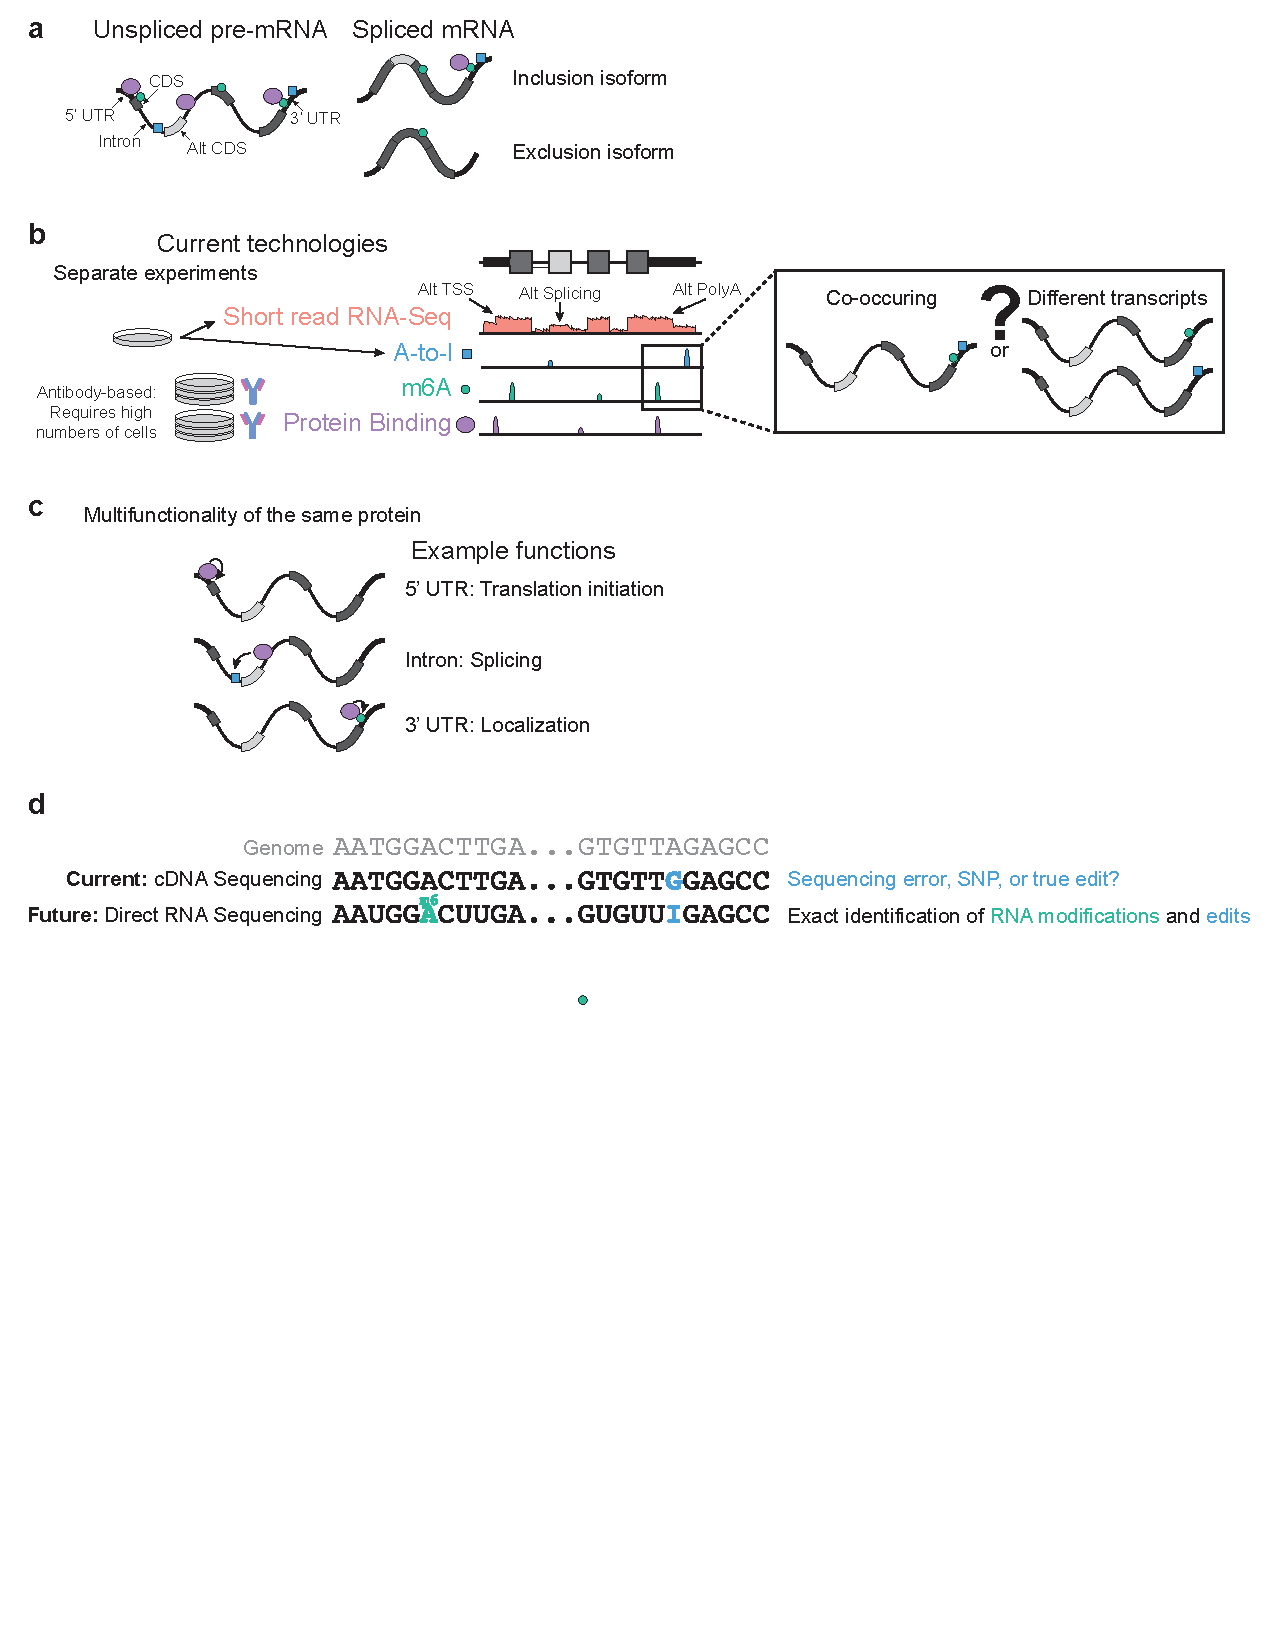
\includegraphics[width=5.8in]{figures/singlecell_future_methods}
  \caption[Unmet needs in RNA processing and potential future technologies.]{Unmet needs in RNA processing and potential future technologies.\\
\textbf{a.}~Left, example RNA transcript with RBPs (purple), A-to-I editing (blue), and m6A (green). Right,  possible inclusion and exclusion isoforms with different post-transcriptional modifications of splicing, m6A, RBP binding, and m6A modification.\\
\textbf{b.}~Current technologies allow for visualization of RNA abundance, A-to-I editing, m6A methylation, and protein binding, but cannot determine whether these occur on physically different or the same molecules.\\
\textbf{c.}~Technologies are needed to investigate multifunctionality of the same protein, e.g. if it performs different functions based on where it binds in the transcripts. Additionally, this would be interesting to study redundancy of different proteins such as splicing factors.\\
\textbf{d.}~Future direct RNA sequencing technologies would allow for direct identification of multiple RNA modifications and edits on the same transcript, unlike currently available technologies.}
\label{fig:singlecell_future_methods}
\end{figure}


Previously, it was thought that there are certain ``uncertainty principles'' in biology, such that one could not know both both the genotype and phenotype of a living cell (Strippoli et al., 2005) or both the cellular ``position'' (current cell state) and ``momentum'' (a cell's past or future, i.e. its lineage or differentiation trajectories) (Shapiro et al., 2013). However, recent work has turned these principles on their head. Both the genotype and phenotype can be measured from a single cell by capturing both DNA and RNA (Macaulay et al., 2015; Reuter et al., 2016), even coupling with measuring DNA methylation and RNA (Angermueller et al., 2016; Hou et al., 2016). A cell's ``position'' and ``momentum'' can be inferred through algorithms that delineate cellular trajectories from phenotypic measurements such as RNA-seq, reviewed thoroughly by (Cannoodt et al., 2016). We expect more technologies to upend traditional thinking of what is possible at the single cell level.

\subsection{Co-occurrence and mutual exclusivity of RNA processing events}

Current technologies to measure transcript abundance and nucleotide modifications, must be performed in separate, bulk experiments, and beyond correlations, the co-occurrence of these [interactions] on the same transcript is unknown (Figure~\ref{fig:singlecell_future_methods}b). Future understanding of the interdependence of RNA processing will require the measurement of multiple aspects of RNA processing at once. This will require is direct RNA sequencing without creation of a cDNA template such as by the Oxford Nanopore MinION (Wanunu et al., 2011) or Pacific Biosciences Single Molecule Real-Time (SMRT) Sequencing (Flusberg et al., 2010). These technologies can directly detect RNA modifications such as m6A and inosine as presence of A-to-I editing (Carr, 2016; Garalde et al., 2016; Saletore et al., 2012). Unfortunately, these technologies are plagued with high error rates and this challenging problem of accuracy for single molecule sequencing will need to be addressed. Nonetheless, as the entire transcript is measured, these would also reveal the co-occurrence on relationships such as between alternative splicing and nucleotide modifications, shedding light on the co-dependence (or independence) of RNA processing elements.
Beyond measuring presence or absence of RNA and its modifications, the interactions of an RNA modification with structure and binding partners will be important. Current methods for measuring RNA secondary structure, typically by selectively measuring only single- or double-stranded RNA, require thousands of cells as input (Bevilacqua et al., 2016; Rouskin et al., 2014; Wan et al., 2011, 2014), thus averaging out the signal across many cells. Scaling these protocols down to single cells will be challenging, it will require tiny amounts of each reaction occurring in nanoliter volumes of captured cells.

\subsection{Spatial analysis: Tissue- and organ-level in vivo}

Disease focus (from Fernando)
ALS
To study ALS, People either extract the entire spinal cord or laser-capture microdissected motor neurons from the spinal cord
Nobody knows what the other cell types do
How are the supporting glia, astrocytes affected in the ALS spinal cords?
Alzheimer's (from Alex Shishkin)
Market size is Billions of dollars
Hematopoiesis (from Fred)
Niches in the body
Responding to immune insults or lesions
Spatial mapping of the cell of origin with the RNA seq
Spatial mapping of gene expression back to 3d position of cells (Achim et al., 2015; Mori et al., 2017)
Ed boyden's methods
Spatial transcriptomics (Ståhl et al., 2016; Vickovic, 2017)
Fixed tissue, barcode each location
Then do sequencing and reconstruct
Long Cai's methods (Frieda et al., 2017; Shah et al., 2016a)
Seurat (Satija et al., 2015)
Used known landmark genes
E.g. for a tumor, shave away the outer layer of cells, sequence, and keep going
How are genes differentially expressed?
Outer layer -- more prone to metastasis
Inner layer -- hypoxic

\subsection{Dynamics/time scale}

Most single-cell technologies are destructive -- once you sample the cell, you can't put it back and see how it responds in a new situation
``Single-cell uncertainty principle'' - similar to the ``uncertainty principle'' of measuring genetics in a living cell (Strippoli et al., 2005)
Originally defined for not knowing both the genotype and the phenotype of a living cell
In cellulo labeling of RNA (Custer and Walter, 2016)
Labels RNA fluorescently without adding much molecular weight


\subsection{Moonshot: Spatial + Dynamics}

Moon shot target: live cell imaging
Temporal dynamics could be measured by tracking RNA molecules with RNA-targeted CRISPR/Cas9 (Nelles et al., 2016), provided the technique scaled to the single molecule level.
Biggest problem: signal amplification

Watch assembly of the spliceosome in nuclear speckles in real time
Watch XIST crawl across the X-chromosome in real time
Step 1: live-cell abundance of one RNA
Cas9 + fluorophore
Step 2: Live-cell imaging of multiple RNAs
Cas9 + multiple fluorophores across several RNAs
Step 3: live-cell imaging of different ends of one RNA
Cas9 + multiple fluorophores at beginning, middle and end of the RNA



\subsection{Single cell multi-omics: One cell, many measurements}

A major problem in the field of high-throughput biology is that as soon as a facet of a molecule is digitized, all other context is lost. For example, measuring RNA may inhibit measuring DNA, and measuring RNA abundance cannot currently be performed simultaneously with investigation of nucleotide modifications. How can cellular context be maximized in a high-throughput manner?
This is a problem because the interplay between genotype and phenotype is lost.

One solution to ameliorate the lost context is simultaneous measurements of multiple categories of molecules. While simultaneous capture of the (epi-)genome and transcriptome have been major breakthroughs (Angermueller et al., 2016; Dey et al., 2015; Hou et al., 2016; Macaulay et al., 2015; Reuter et al., 2016), there are many more aspects of cellular state that are still invisible to the sequencing eye.
Effect of non-RNA on RNA processing - e.g. DNA (chromatin, structure, SNPs) on RNA Processing (quantitative trait loci - QTLs)
Chromatin modifications and their effect on transcription speed and alternative splicing
Quantitative trait loci - SNPs + RNA processing
For example, abundances of proteins or metabolites in conjunction with RNA would provide a fuller picture of cellular state.
E.g. does presence of certain sugars or signaling molecules co-occur with certain RNAs? Discovery of novel signaling pathways
Chromatin structure, along time 4D nucleome (Dekker et al., 2017)
Post-translational modifications of proteins (phosphorylation, glycosylation)
RBPs are glycosylated
Does an RBP bind different regions, perform different functions, or interact with different proteins, when it is differentially glycosylated?
Time scale: phosphorylation can be on the order of seconds

Another method to create additional context for each individual cell is to combine high-throughput measurements with genome editing such as with CRISPR/Cas9, allowing for dissection of complex phenotypes in mammalian cells at large scales. For example, Perturb-seq is a method that combines knockdown of genes using CRISRPi with single-cell RNA-seq, and was used to study the unfolded protein response (Adamson et al., 2016) and effect of lipopolysaccharides on dendritic cells (Dixit et al., 2016). This created a computational scientist's dream dataset, as for each gene that was knocked down, there was a control dataset, and thus for developing algorithms, one could always have a negative control to check with. Perturb-Seq could be applied to study any aspect of RNA processing, e.g. systematically knocking down all protein components of the spliceosome or different alternative splicing factors.
Another possibility is coupling RNA-seq with lineage-specific barcodes through genome editing by CRISPR/Cas9 (McKenna et al., 2016). This would allow for comparing the transcriptomes of cells from similar lineages. Using phylogenetic techniques, cell lineages could be reconstructed and even the times at which cells asymmetrically divided to change fates could be found. If RNA-seq encodes a cell's present, then its traced lineage encodes its past. This lineage tracing method, coupled with direct RNA sequencing, would help to understand how developmentally regulated RNA processing events such as RNA editing, m6A, and alternative splicing, are finely tuned in different lineages. Do all cells that were committed to a particular lineage also have certain RNA processing events? This could indicate inheritability of the event, either encoded through the genome or by asymmetrically dividing the RNA content of a mother cell.


\section{Discussion}

Previous ‘single-cell' studies were limited to microscopy and other visual tools
Ultimately, ‘single-cell biology' is ‘biology'
Each RNA lives a rich, fulfilled life, and this is difficult to measure through single-cell techniques due to technical limitations.
Many questions remain
How do the many transient aspects of RNA, such as nucleotide modifications, binding partners, 3D structure, and localization, affect each other?
So far has been studied for one transcript, a few modifications
May not even know to study the co-interaction between these aspects on a particular transcript
